\section{Eye and Human Vision}
This section is non-examinable, and will be brief for the purpose of background.

\subsection{Human Eye}
\begin{itemize}
    \itemsep0em
    \item Evolved for survival
    \item Function of the eye is to form an image on the retina
    \item The lens is shaped using the ciliary muscle, it is not moved.
    \item The image is transmitted via the optic nerbe
\end{itemize}
Following image formation, the image must be inverted. \\

There are a variety of sensors: Cones (photopic $10^7$) and Rods ($10^8$ scotopic). Cones have three different types, based on wavelength: Short (blue), Medium (Green), Long (red). The spectral response for each wavelength varies, with short wavelengths having a poor spectral response, medium wavelengths having the best spectral response, and long wavelengths having an interpolated response between short and medium wavelengths.

\subsection{Mach Bands}
Mach bands are a result of brightness adaption, and occur due to the eye forming boundaries between different shades of a distinct black-white colour gradient. The seen response overshoots between colour bands and a border appears between the elements in the colour gradient.

\subsection{Neural Processing}
Sensor information is combined by using a variety of weighting functions. Given a weighting function $w$, sensor $P_{1}$, and a variety of other sensors $P_{2}, ... P_{N}$, we can simulate processing:

\begin{align}
    P_{1} -> log(P_{1}) -> w_{1} \times log(P_{1}) \\
    P_{n} -> log(P_{n}) -> w_{n} \times log(P_{n}) \\
    \sum_{1}^{n} w_{n} \times log (P_{n})
\end{align}

Webers law, the difference threshold, is the minimum amount by which stimulus intensity must be changed is the minimum amount by which stimulus intensity must be changed in order to produce a variation in sensory experience.

\subsection{Summary}
\begin{itemize}
    \itemsep0em
    \item [1] The human eye can be modelled in three sections
    \item [2] It is very effective but can be deceived
    \item [3] Is it a good model for computer vision?
\end{itemize}

\section{Image Formation}

\subsection{Image Decomposition}
Images can be decomposed into their individual bits, from bit $0$ to bit $7$. The most significant bit carries the most information, and as the bits decrease in significance, more noise is introduced. Some bits are used for lighting. \\
High resolution images contain more information, and implies that more storage is required, given $N \times N$ points. An appropriate value of $N$ is determined by use case.

\subsection{Fourier Transform}
Essentially, the Fourier transforms an addition of signals from the time domain to the frequency domain. Each individual frequency from the addition of signals in the time domain, is visible in the frequency domain.

We can describe the fourier transform as follows:

\begin{equation}
    Fp(f) = \mathcal{F}(p(t)) = \int_{-\infty}^{\infty}p(t)e^{-jft}dt
    \label{eq:fourier}
\end{equation}

\subsubsection{Derivation}

An explanation of \ref{eq:fourier} is given through the following derivation, based on the fact that: a() \text{ is a function of time variant signal } p(t):

\begingroup
\addtolength{\jot}{1em}
\begin{align*}
    \text{The FT is then } Fp &= a(p(t)) \\
    \text{FT is a function of frequency } Fp(f) &= a(p(t)) \\
    \text{This can be written as: } \mathcal{F}(p(t)) &= a(p(t)) \\
    \text{a() is an integral } \mathcal{F}(p(t)) &= \int_{-\infty}^{\infty}p(t)cas(t)dt \\
    cas = \text{cos and sin } e^{-jft} &= cos(ft) - \textit{j}sin(ft) \\
    \mathcal{F}(p(t)) &= \int_{-\infty}^{\infty} p(t)e^{-jft}dt
\end{align*}
\endgroup

\subsubsection{Application}
Given a pulse signal, the following evaluation can be made.
We can apply the piecewise pulse function, and evaluate the integral given the conditions of the pulse.
\begin{align}
    p(t) = \begin{cases}
            A & \text{if} -T/2\leq t \leq T/2 \\
            0 & \text{otherwise}
            \end{cases} \\
    \mathcal{F}p(\omega) = \int_{T/2}^{-T/2}Ae^{-jwt}dt \\
    \mathcal{F}p(\omega) = - \frac{Ae^{-jw\frac{T}{2}} - Ae^{jw\frac{T}{2}}}{j\omega} \\
    \mathcal{F}p(\omega) = \begin{cases}
                         \frac{2A}{\omega}\sin{\frac{\omega T}{2}} & \text{if } \omega \neq 0 \\
                         AT & \text{if } \omega = 0 
                            \end{cases}
\end{align}

\newpage

This is demonstrated visually in: (\ref{fig:fourier})

\begin{figure}[h!]
    \centering
    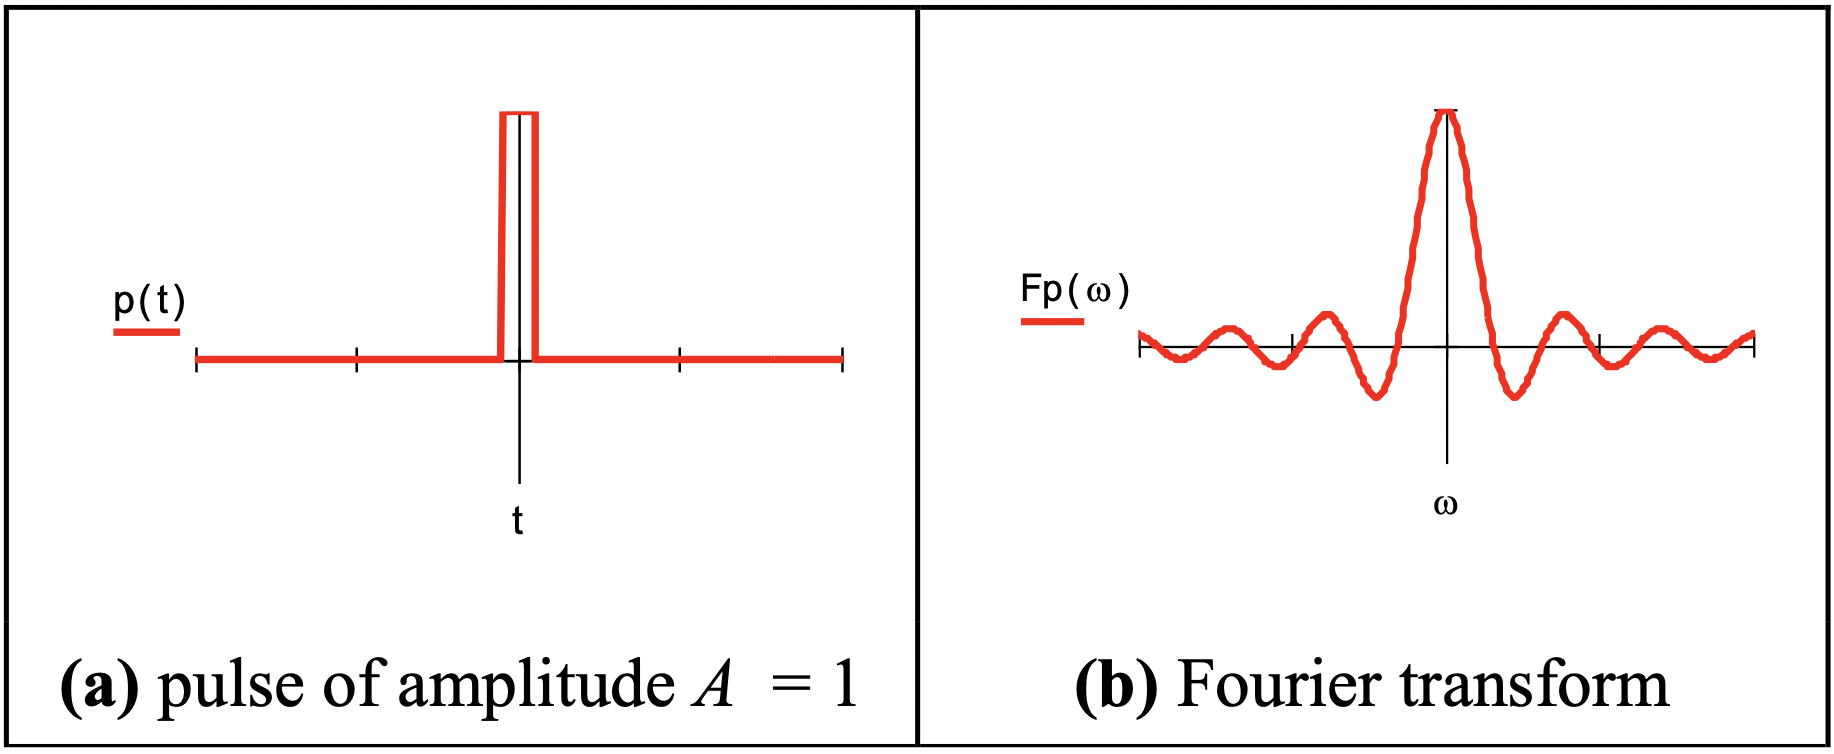
\includegraphics[scale=0.2]{Images/fourier.png}
    \caption{Fourier transform of a pulse}
    \label{fig:fourier}
\end{figure}

The Fourier transform signal can be reverted back to the time domain using the inverse Fourier transform. We can select a variety of angular frequencies: $range(-6,6)$. The reconstruction by integration is then:

\begin{equation}
    F(t) = \int_{-6}^{6} \mathcal{F}p(\omega)e^{jwt}d\omega
\end{equation}

\subsubsection{Magnitude and Phase of Fourier Transform}
We can split the Fourier transform by its real and imaginary parts:
\begin{equation}
    \mathcal(F)p(\omega) = \int_{-\infty}^{\infty}p(t)e^{-jwt}dt = Re(\mathcal{F}p(\omega)) + \textit{j}Im(\mathcal{F}p(\omega))
\end{equation}

From this, we can then proceed to calculate the magnitude and the phase.

Magnitude
\begin{equation}
    |\mathcal{F}p(\omega)| = \sqrt{Re(\mathcal{F}p(\omega))^{2} + Im(\mathcal{F}p(\omega))^{2}}
\end{equation}

Phase
\begin{equation}
    arg(\mathcal{F}p(\omega)) = \arctan \left( \frac{Im(\mathcal{F}p(\omega))}{Re(\mathcal{F}p(\omega))}
    \right)
\end{equation}

\subsubsection{Additional}

The Fourier transform is used for coding images. We can quantise the frequency transform, then code the information from the quantised image. We can then reconstruct the image, to get a sampled result.